\chapter{HeROsim : Élaborer et évaluer des politiques d'orchestration pour le cloud privé}

\section{Introduction}
\label{section:herosim-introduction}

Serverless computing unlocks the potential for finely-tuned optimization of resource usage. In such a model, developers design their applications as a composition of stateless functions which execution is event-driven. %~\cite{SchleierSmith2021WhatSC}. 
Customers are billed according to their actual resource usage, and providers are responsible for deploying intelligent resource management to optimize Quality of Service (QoS) metrics such as response time and energy consumption.%, and resource usage.

%Serverless enables rapid elasticity and a measured service at the finest granularity. 

%On the service provider's side, the double responsibility of dynamic resource allocation and task placement leaves the door open for optimization opportunities. 


Serverless comes with a bag of challenges that need to be addressed by service providers. For example, the latency overhead caused by dynamically allocating hardware for new function instances, called a cold start delay, is a a key issue~\cite{Lannurien2023}. Another recurring problem is the data-shipping architecture, where gigabytes of data remotely stored are pulled toward kilobytes of code on the compute nodes%~\cite{yuFollowingDataNot}
, leading to dramatic performance degradation.

Overcoming such challenges requires devising orchestration policies that guide autoscaling and scheduling decisions.
Orchestration is a dynamic process: each decision creates a new state for the system, leading to combinatorial explosion. Moreover, serverless platforms are generic software that expose many knobs for the provider to tweak. These settings can impact user request latency, platform throughput, datacenter resource usage, and energy consumption. As it is costly to experiment in production, we argue that simulation tools are instrumental for private serverless cloud providers looking to optimize these QoS metrics.% with regards to their own objectives.

%\ob{As with all solutions for exploring a huge space of solutions, there is no single solution, no single strategy that can be applied without taking into account which functions need to be executed, on which data, in which execution context (cluster topology, function being executed, ...). }

%These policies must be evaluated with regard to their relevance in various use cases. Different metrics can be of use for this evaluation, \textit{e.g.} makespan for a given scenario, function response time, dynamic and static energy consumption, etc.

%There are two possible ways to assess if the policies we devise have a positive impact on these metrics: simulation (estimate) or implementation (measure). There is a tradeoff between time and precision in the two approaches; choosing simulation over implementation allows fast exploration of the problem space and iteration over possible solutions. % at the expense of...

% Discrete-event modeling allows us to explore solutions by representing the different components of the platform with processes that model the state of the system and its evolution over time.


% serverless : on veut tracer les événements d'allocation/déallocation + les événements de placement de tâches, à la granularité la plus fine pour comprendre chacune des décisions
% applications : on veut modéliser des dépendances temporelles/de données entre les invocations de fonctions
% cloud privé : on veut voir précisément quelles ressources sont mobilisées
% QoS : on veut pouvoir différencier les besoins utilisateur à la granularité d'une requête
% qualité des politiques : on veut pouvoir comparer différentes politiques d'orchestration au regard de métriques de QoS

%\vl{premier jet ci-dessous :}

Simulation tools for orchestration policies in private serverless cloud need to allow tracing resource allocation events and task placement events at the \textbf{finest granularity}, in order to understand the impact of policies on performance metrics. To represent realistic use cases, the software must offer the possibility of modeling applications that exhibit \textbf{data and temporal dependencies between task executions}. Furthermore, the simulator needs to support the \textbf{heterogeneity} of cloud computing: on the one hand, datacenters are made of various hardware that exhibit different levels of cost and performance; on the other hand, there is a wide range of customers with \textbf{different QoS requirements}. Finally, the simulator should be able to \textbf{replay execution traces} for different orchestration policies and \textbf{compare the outcomes} in terms of QoS metrics under each evaluated policy.

Previous work proposed different interesting simulation tools for the cloud, see Table~\ref{table:herosim-sota}. Some of these do not target the serverless paradigm~\cite{calheiros_cloudsim_2011, wickremasinghe_cloudanalyst_2010, cai_elasticsim_2017, buyyaGridSimToolkitModeling2002, nunez_icancloud_2012, mahmudIFogSim2ExtendedIFogSim2021}. Among serverless simulators, some focus on public cloud offerings~\cite{nunez_icancloud_2012, mahmoudiSimFaaSPerformanceSimulator2021}, mainly to allow devising hybrid strategies where part of the workloads are offloaded to cheaper public cloud. For private clouds, some simulators do not consider energy consumption~\cite{jeonCloudSimExtensionSimulatingDistributed2019, cai_elasticsim_2017, buyyaGridSimToolkitModeling2002, nunez_icancloud_2012}; others do not take hardware heterogeneity into account~\cite{jeonCloudSimExtensionSimulatingDistributed2019, nunez_icancloud_2012, mahmoudiSimFaaSPerformanceSimulator2021}. Most simulators do not allow modeling applications composed of multiple functions with data dependencies~\cite{calheiros_cloudsim_2011, mampage_cloudsimsc_2023, wickremasinghe_cloudanalyst_2010, jeonCloudSimExtensionSimulatingDistributed2019, buyyaGridSimToolkitModeling2002, nunez_icancloud_2012, mahmudIFogSim2ExtendedIFogSim2021}. In certain studies, QoS cannot be enforced at the granularity of a single-user request~\cite{calheiros_cloudsim_2011, mampage_cloudsimsc_2023, wickremasinghe_cloudanalyst_2010, cai_elasticsim_2017, nunez_icancloud_2012, mahmudIFogSim2ExtendedIFogSim2021, mastenbroekOpenDCConvenientModeling2021, mahmoudiSimFaaSPerformanceSimulator2021}. % Finally, few simulators target emerging serverless paradigms that represent the state of available platforms~\cite{jeonCloudSimExtensionSimulatingDistributed2019}. 
% To address these limitations, we propose \textbf{HeROsim}~\cite{herosim}, a simulator~\footnote{We used the SimPy~\cite{simpy} library (MIT licensed) for the discrete-event simulation engine.} that models a generic serverless platform. The software design given in Figure~\ref{figure:herosim-software-architecture} follows the reference architecture of state-of-the-art orchestrators such as Google Knative~\cite{knative} or Apache OpenWhisk~\cite{openwhisk}. Such orchestrators consist of two main modules:

To address these limitations, we propose \textbf{HeROsim}~\footnote{\href{https://github.com/b-com/HeROsim}{https://github.com/b-com/HeROsim}}, a free and open source \textbf{He}terogeneous \textbf{R}esources \textbf{O}rchestration \textbf{sim}ulator with the following features:

%\ob{annonce ici la contribution du papier en une phrase ou deux.
%C'est quoi la contribution visé, June présentation de l'architecture ? Si oui, comment tu évalues sa qualité... }

%\vl{premier jet ci-dessous :}

\begin{itemize}
    \item Fine-grained description of serverless applications on heterogeneous hardware.%: performance, data flow, memory requirements, energy consumption.
    \item Dynamic allocation of hardware resources and placement of QoS-enabled user requests.%: HeROsim offers entry points for users to implement their own policies for resource selection.
    \item Evaluation of orchestration policies according to QoS metrics such as latency and energy. %: HeROsim allows comparing the results of different strategies with regards to some popular QoS metrics.
\end{itemize}

%The software design follows the reference architecture of state-of-the-art orchestrators such as Google Knative~\footnote{\href{https://knative.dev}{https://knative.dev}} or Apache OpenWhisk~\footnote{\href{https://openwhisk.apache.org}{https://openwhisk.apache.org}}. Such orchestrators consist of two main modules:

% \begin{itemize}
%     \item The \textbf{autoscaler} determines how to automatically and reactively scale hardware resources in a cloud in adequacy with the applications' load.
%     \item The \textbf{scheduler} determines on which replica to queue user requests for a given function according to QoS requirements.
% \end{itemize}

% \vl{déplacer cette dernière phrase dans la conclusion ? mais comment "conclure l'introduction" ?}

% HeROsim allows researchers to model heterogeneous cloud infrastructures, describe workloads at a fine granularity, implement diverse resource management and task scheduling policies, and evaluate their efficiency with regards to metrics such as resource usage, energy consumption, per-request QoS violations or tail latency. HeROsim can generate charts that help visualizing these results during the implementation phase, and can be used in publications.

%The article is organized as follows: the first section gives an overview of the workings of a serverless platform; the next section details the design of HeROsim; the "Case study" section shows how HeROsim can be leveraged through two use cases from our previous publications; then we discuss state-of-the-art work; and finally, we conclude the paper.
% Section~\ref{section:herosim-overview} gives an overview of the workings of a serverless platform; Section~\ref{section:herosim-herosim} details the design of HeROsim and describes the flow of a simulation run using our tool; Section~\ref{section:herosim-case-study} shows how HeROsim can be used through two use cases from our previous publications; Section~\ref{section:herosim-sota} discusses state-of-the-art work; finally, Section~\ref{section:herosim-conclusion} concludes the paper by giving some perspectives for future work.

%\vadjust{\pagebreak}

%\vspace*{-10pt}

\section{Présentation générale de la plateforme simulée}
\label{section:herosim-overview}

% \vl{premier jet de figure générale... à revoir : passage de la plateforme à l'infrastructure. reprendre la figure HeROcache ?}

\begin{figure*}[t]
    \centering
    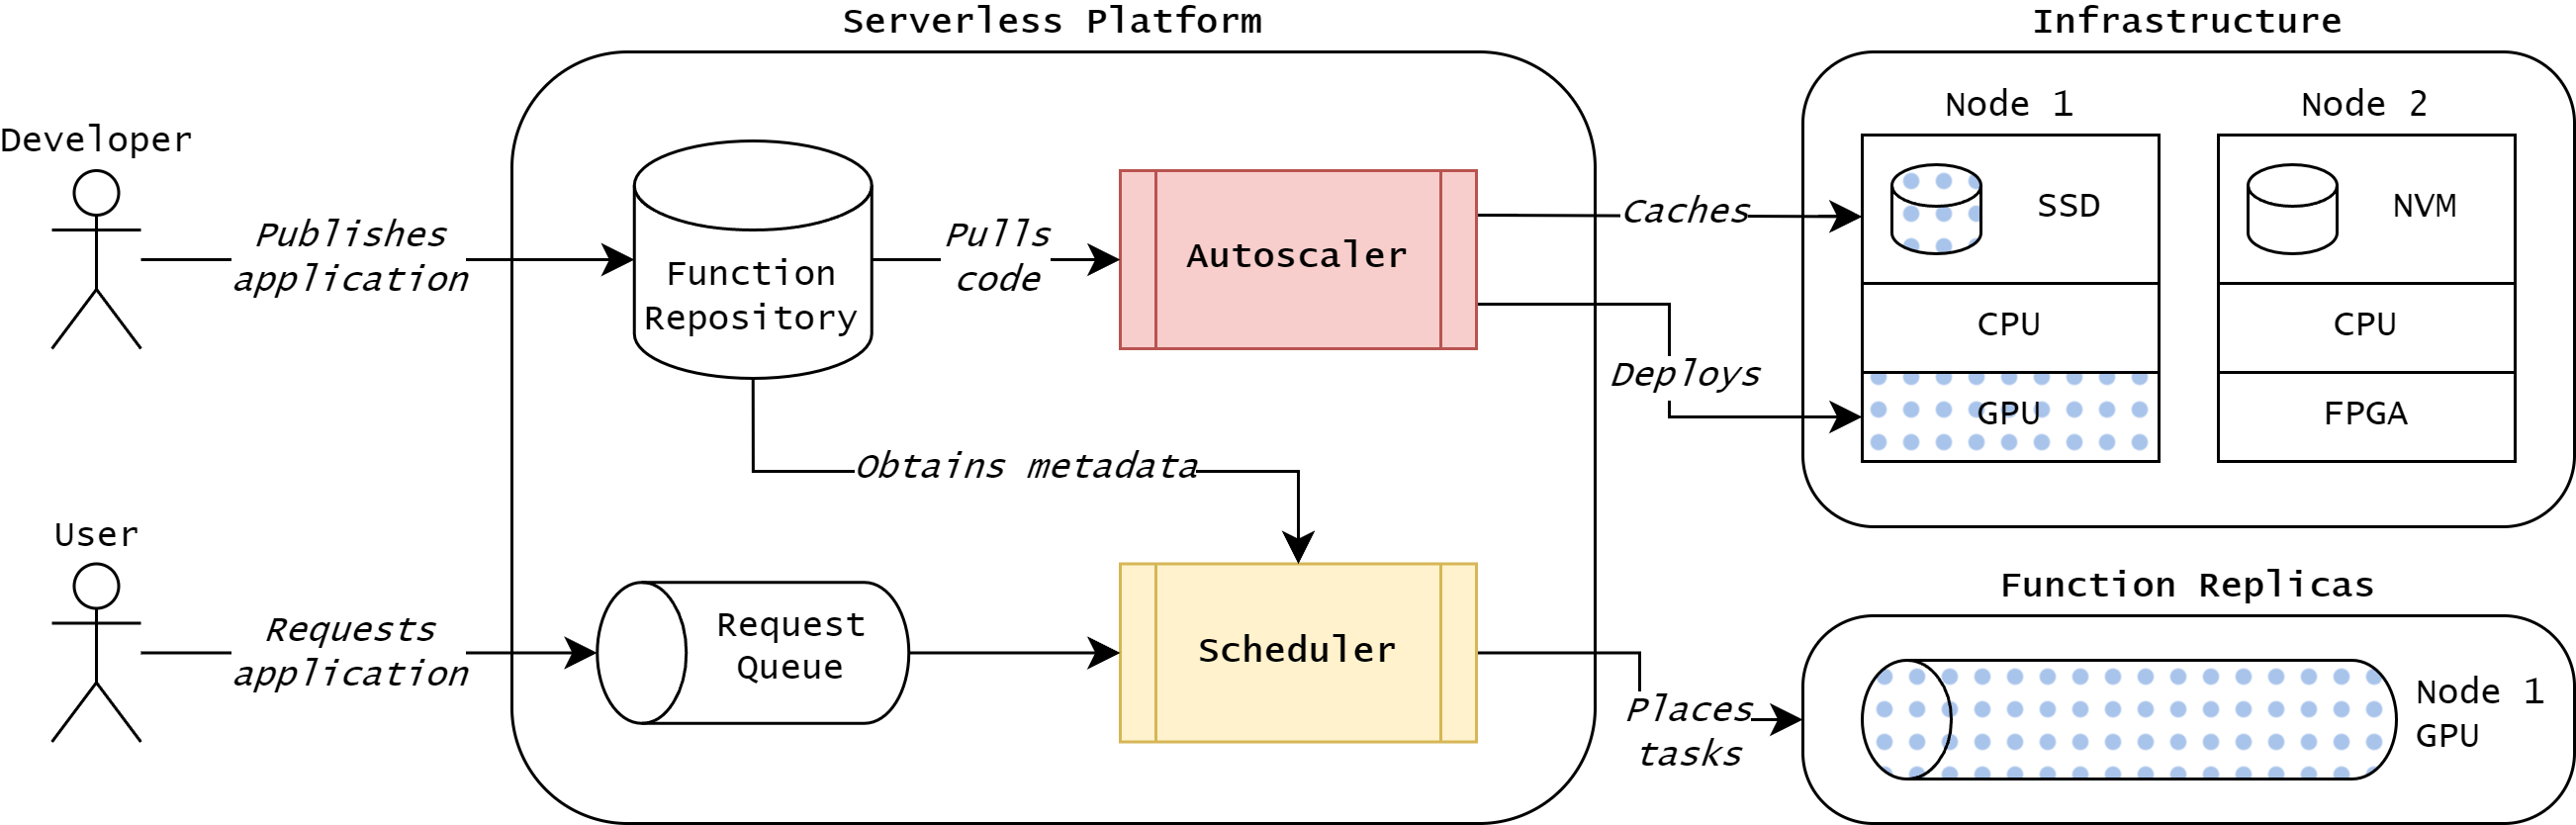
\includegraphics[width=0.9\textwidth]{7_Chapitre5/figures/platform.png}
    \caption{High-level view of a serverless platform, as modeled in HeROsim. The autoscaler allocates hardware resources for function replicas; while the scheduler places user requests in queue on those replicas.}
\label{figure:herosim-platform}
\end{figure*}

% Cloud infrastructure


%In cloud computing, customers typically book resources. These are usually a virtualized subset of heterogeneous hardware resources available on servers called nodes. Once the reservation has been made, service providers deliver remote access to the customer, who is responsible for the deployment of their applications and billed according to the amount of resources they reserved~\cite{Lannurien2023}.

% Functions, applications
In the serverless paradigm, customers start by pushing their code to a repository on the provider's side, see Figure~\ref{figure:herosim-platform}. %The provider allocates resources that are automatically scaled according to the load. 
For this mechanism to work, applications are divided into small steteless execution units called \textbf{functions}. %These functions are stateless~\cite{yuFollowingDataNot}. %: Should they produce any output data, these must be kept in persistent storage~\cite{yuFollowingDataNot}.

% Space-sharing, time-sharing -- different models
%In traditional service models, resources are scaled across two dimensions: horizontally (new application instances created on further nodes) and vertically (additional resources allocated to existing instances). 
In serverless platforms, resources are scaled horizontally: variations in load on applications are absorbed by adding new instances of the functions, called \textbf{replicas}, and removing them when no longer needed. A replica can be created for each user request or reused for multiple user requests. We can consider function replicas as request queues with different capacities.

% Autoscaler types (scale to zero, horizontal/vertical...)
These replicas are created by the \textbf{autoscaler}. To manage the number of replicas deployed for each function, there are three main strategies: request-based, concurrency-based, and metrics-based~\cite{mahmoudiSimFaaSPerformanceSimulator2021}. In request-based autoscaling, requests coming in the system are handled by idle replicas. If no idle replica is available, a new instance is created. In concurrency-based autoscaling, each replica can queue multiple user requests and handle them sequentially according to a predefined concurrency threshold~\cite{herofake}. In metrics-based autoscaling, the number of deployed replicas depends on various objectives, such as the request rate per second (RPS) to meet. %This requires monitoring the performance of the system for use by the autoscaler.

% Replica (function instance) state (initializing, running, idle)
Replicas can be in three different states: initializing, running, and idle.%~\cite{SchleierSmith2021WhatSC}. 
When a function replica has just been created, it is in initializing state: the platform instantiates its execution environment, pulls its code from a remote registry and optionally caches it on the deployment node, and starts executing the function. When the replica handles user requests, it is in running state. Otherwise, the replica is idle, and can be removed.
% Cold start problem, warm start, data-shipping architectures
When replicas are removed, hardware resources are freed. However, when a new replica is created to handle user requests, this incurs an overhead called a \textbf{cold start}. Orchestrators adopt various policies to mitigate this issue.% ranging from enforcing a keep-alive period on function replicas to avoid destroying them too early, to proactively allocating replicas.

% Scheduler policies (bin-packing, load balancing...)
Finally, user requests are mapped to the available function replicas by the \textbf{scheduler} that implements different strategies: for example AWS Lambda\footnote{\href{https://aws.amazon.com/en/lambda/}{https://aws.amazon.com/en/lambda/}} uses a bin-packing algorithm, while an open source platform such as Knative implements a load balancing policy~\cite{Lannurien2023}. %These strategies have different outcomes with regard to resource usage and QoS, but it can be difficult to predict to what extent they will impact workloads before deployment.

\section{Choix de conception}
\label{section:herosim-herosim}

%This section introduces the design choices and hypotheses made for the development of HeROsim.%, in order to help users get started implementing their own policy in simulation.

% \begin{figure}[t]
%     \centering
%     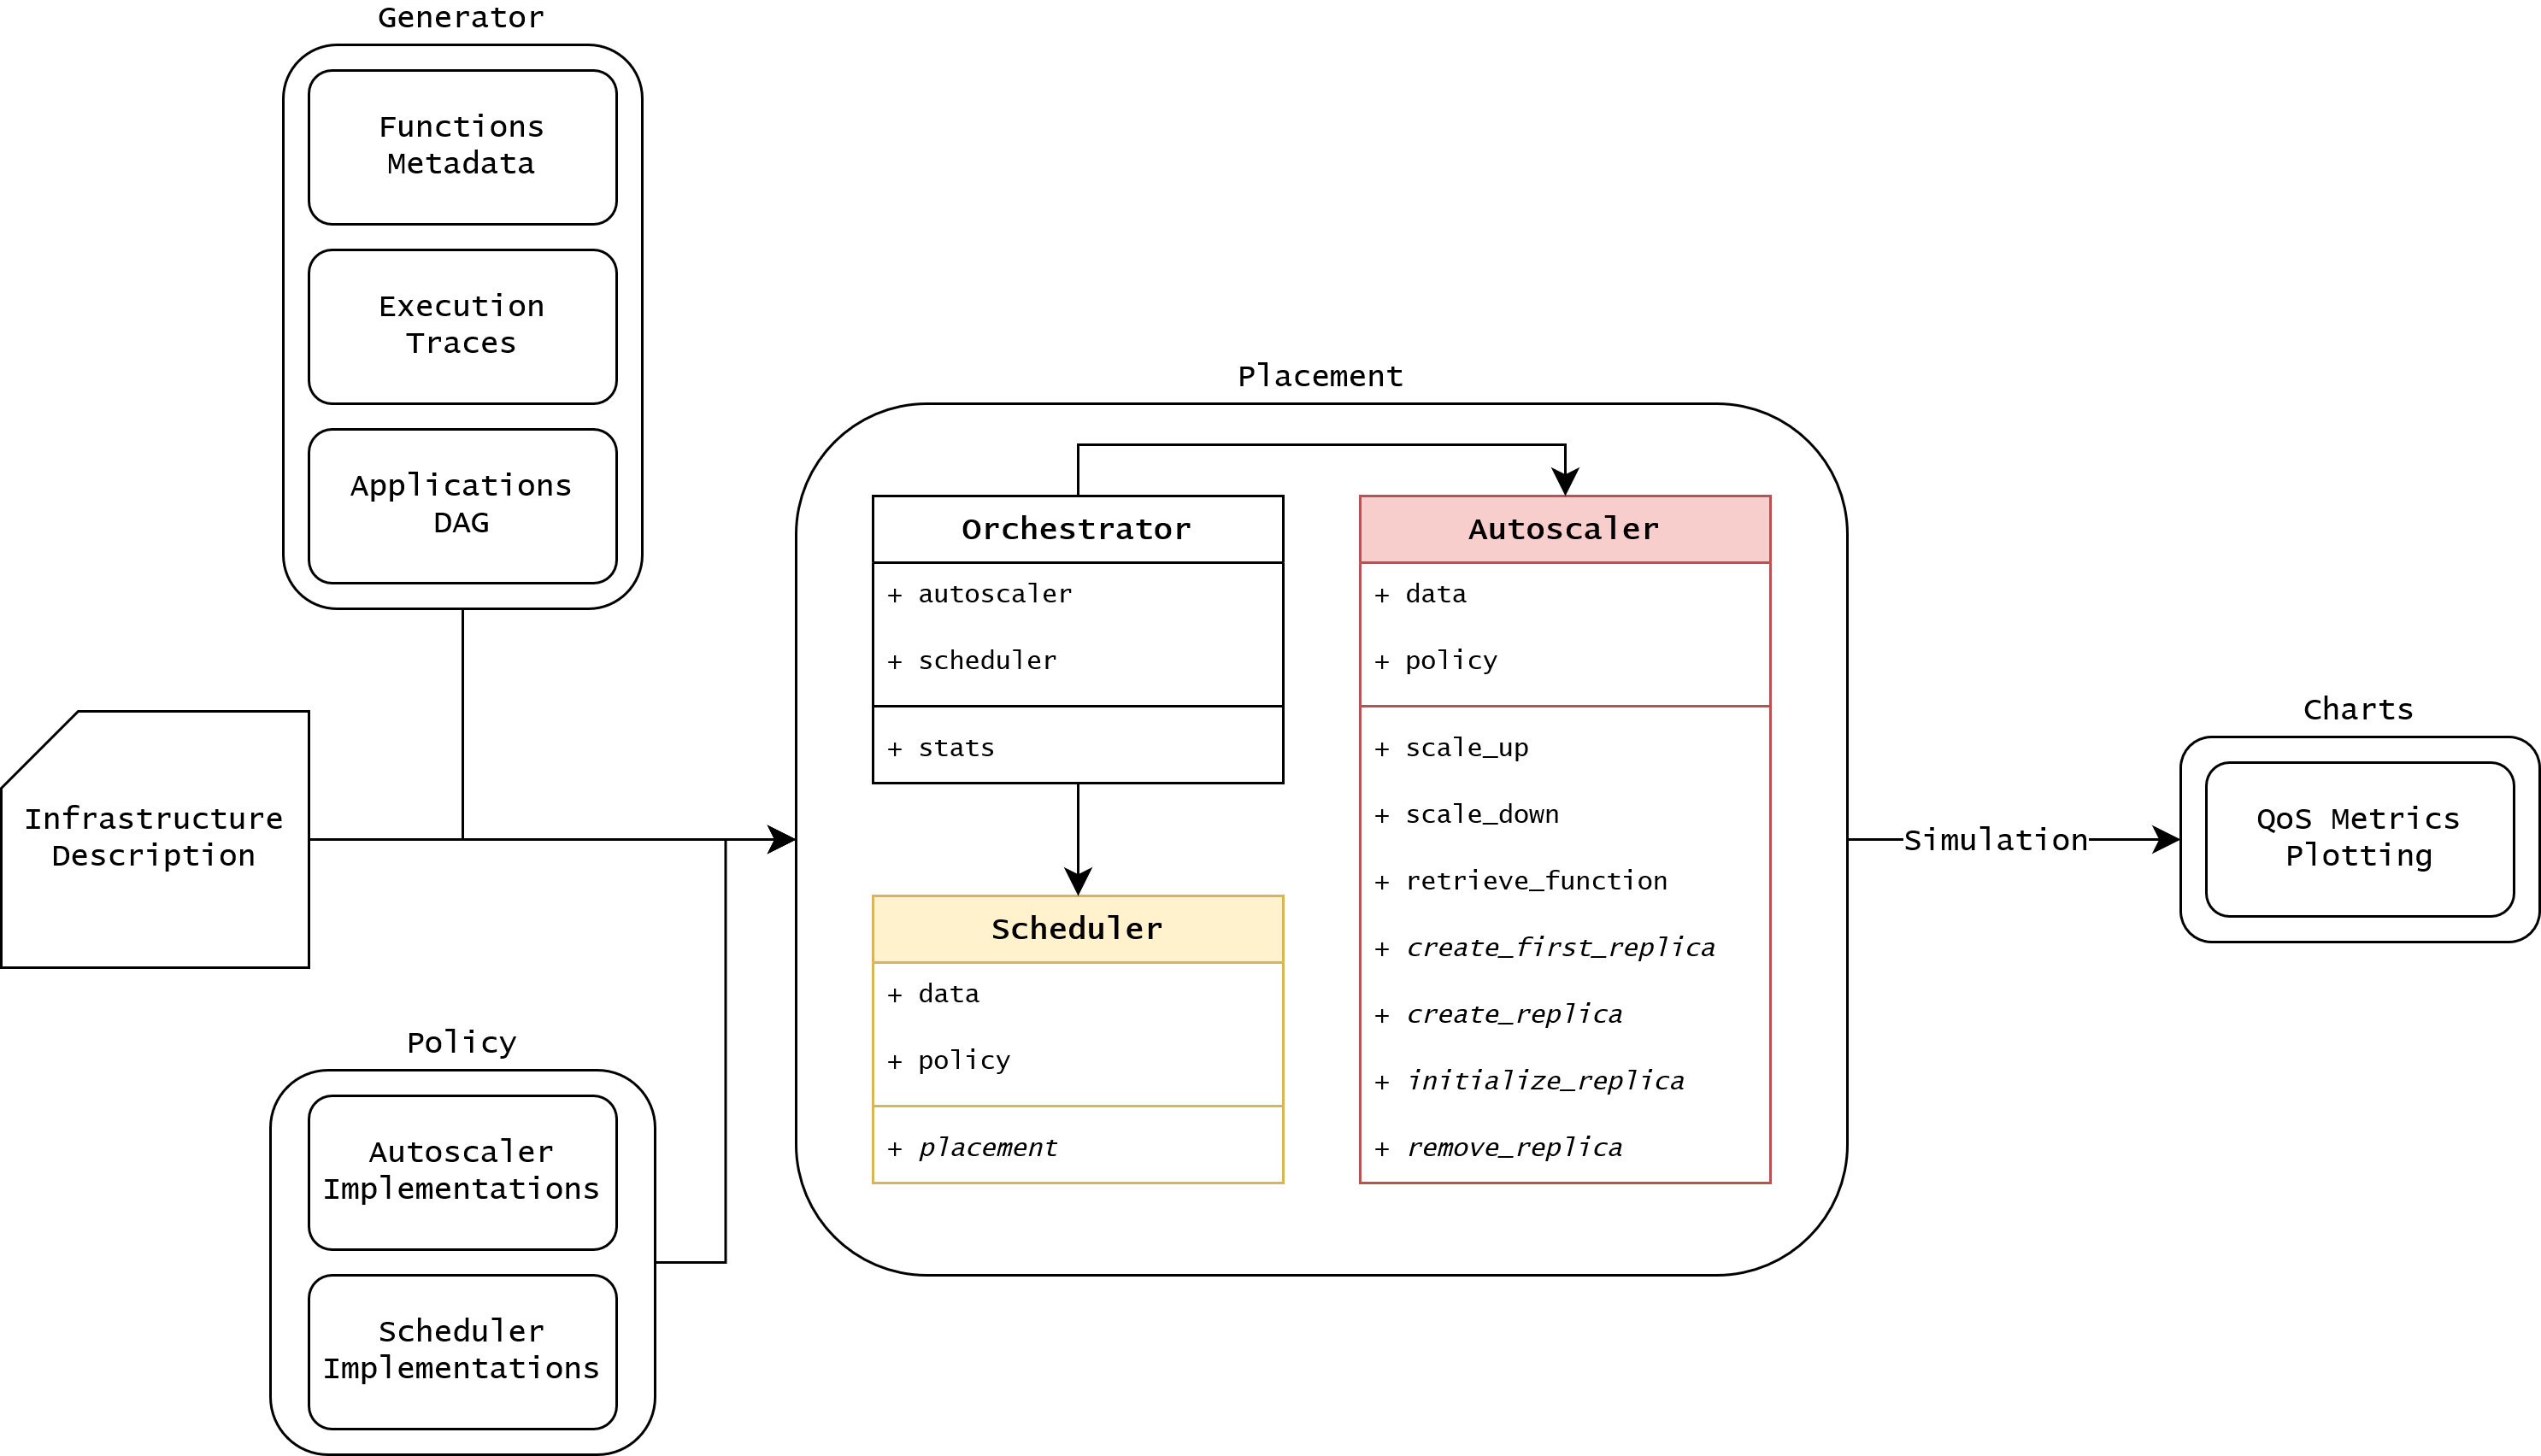
\includegraphics[width=\columnwidth]{7_Chapitre5/figures/software-architecture.png}
%     \caption{FIXME: High-level view of the simulator's architecture \jb{illisible}}
% \label{figure:herosim-software-architecture}
% \end{figure}

HeROsim uses the SimPy~\footnote{\href{https://simpy.readthedocs.io}{https://simpy.readthedocs.io}} library as the discrete-event simulation engine. It ships three base classes -- \texttt{Orchestrator}, \texttt{Autoscaler} and \texttt{Scheduler} -- that should be subclassed by users willing to implement their own  algorithms. As the bulk of the platform behavior is inherited from the base classes, implementation overhead for a new policy is minimal: the simplest couple of autoscaler and scheduler (Random Placement policy) are implemented in less than 20 LOCs.

\subsection{Données d'entrée}

HeROsim exposes a declarative interface for users to define their cloud environment, workloads and QoS constraints. The simulator replays an allocation and placement scenario under different orchestration policies. A simulator run requires the following JSON inputs to define such a scenario:

\begin{enumerate}
    \item A \textbf{workload description}; details on the \textbf{characteristics of the functions}  invoked during the scenario, \textit{i.e.} their execution time and cold start time, memory requirements, energy consumption, image size, input and output data size These metadata could be defined by \textbf{measuring} and \textbf{analyzing} the applications' behavior on a testbed configuration. % (see Figure~\ref{figure:herosim-characterization}).
    \item An \textbf{infrastructure description}; the listing of the different \textbf{nodes available}, their different hardware execution platforms, storage devices, network bandwidth. Execution platforms are defined in terms of idle energy consumption and retail price; storage devices are characterized by their capacity, bandwidth, and latency. These data are specific to a target platform and could be \textbf{measured} or obtained from manufacturers.
    \item An \textbf{execution trace}; the arrival times for all \textbf{user requests} to the applications, associated with their desired QoS level, in chronological order. These data can be extracted from real-world \textbf{observations} of the applications in production, or statistically estimated. % (see Figure~\ref{figure:herosim-characterization}), or statistically estimated. 
\end{enumerate}

Data from our previous studies~\cite{herofake, herocache} are available in the repository for reference. While (1) and (2) can be hand-written according to the use-case requirements, HeROsim provides a synthetic generator to create various traces for (3) using Poisson processes, with variable duration and user request rate, as commonly done in the literature~\cite{herocache}. 

\subsection{Flot d'une simulation}

The user may choose the desired orchestration policies and execute the main program. The simulator will:

\begin{itemize}
    \item Initialize the infrastructure as described: the scenario starts with all the nodes idle, waiting for new requests.
    \item Initialize the orchestrator with chosen autoscaler and scheduler.
    \item Follow the arrival times of events from the execution trace, and pass the user requests to the orchestrator.
    \item Let the scheduler try to place these requests on function replicas.
    \item Let the autoscaler allocate and deallocate hardware resources that host these replicas to handle user requests.
\end{itemize}

% The simulation advances on \textbf{task executions}, \textit{i.e.} when functions are scheduled \jb{bizarre cette phrase}\vl{et comme ça ?}.

The simulation advances on handling user requests. The simulator knows the functions' response time based on the input metadata. % metadata measured beforehand. These metadata concern the specific hardware and workloads the user is interested in scheduling. They can be obtained in many ways; Figure~\ref{figure:herosim-characterization} shows an overview of the methodology we used to characterize various workloads and execution platforms throughout our experiments; see~\cite{herofake, herocache} for more details.

% \begin{figure}[t]
%     \centering
%     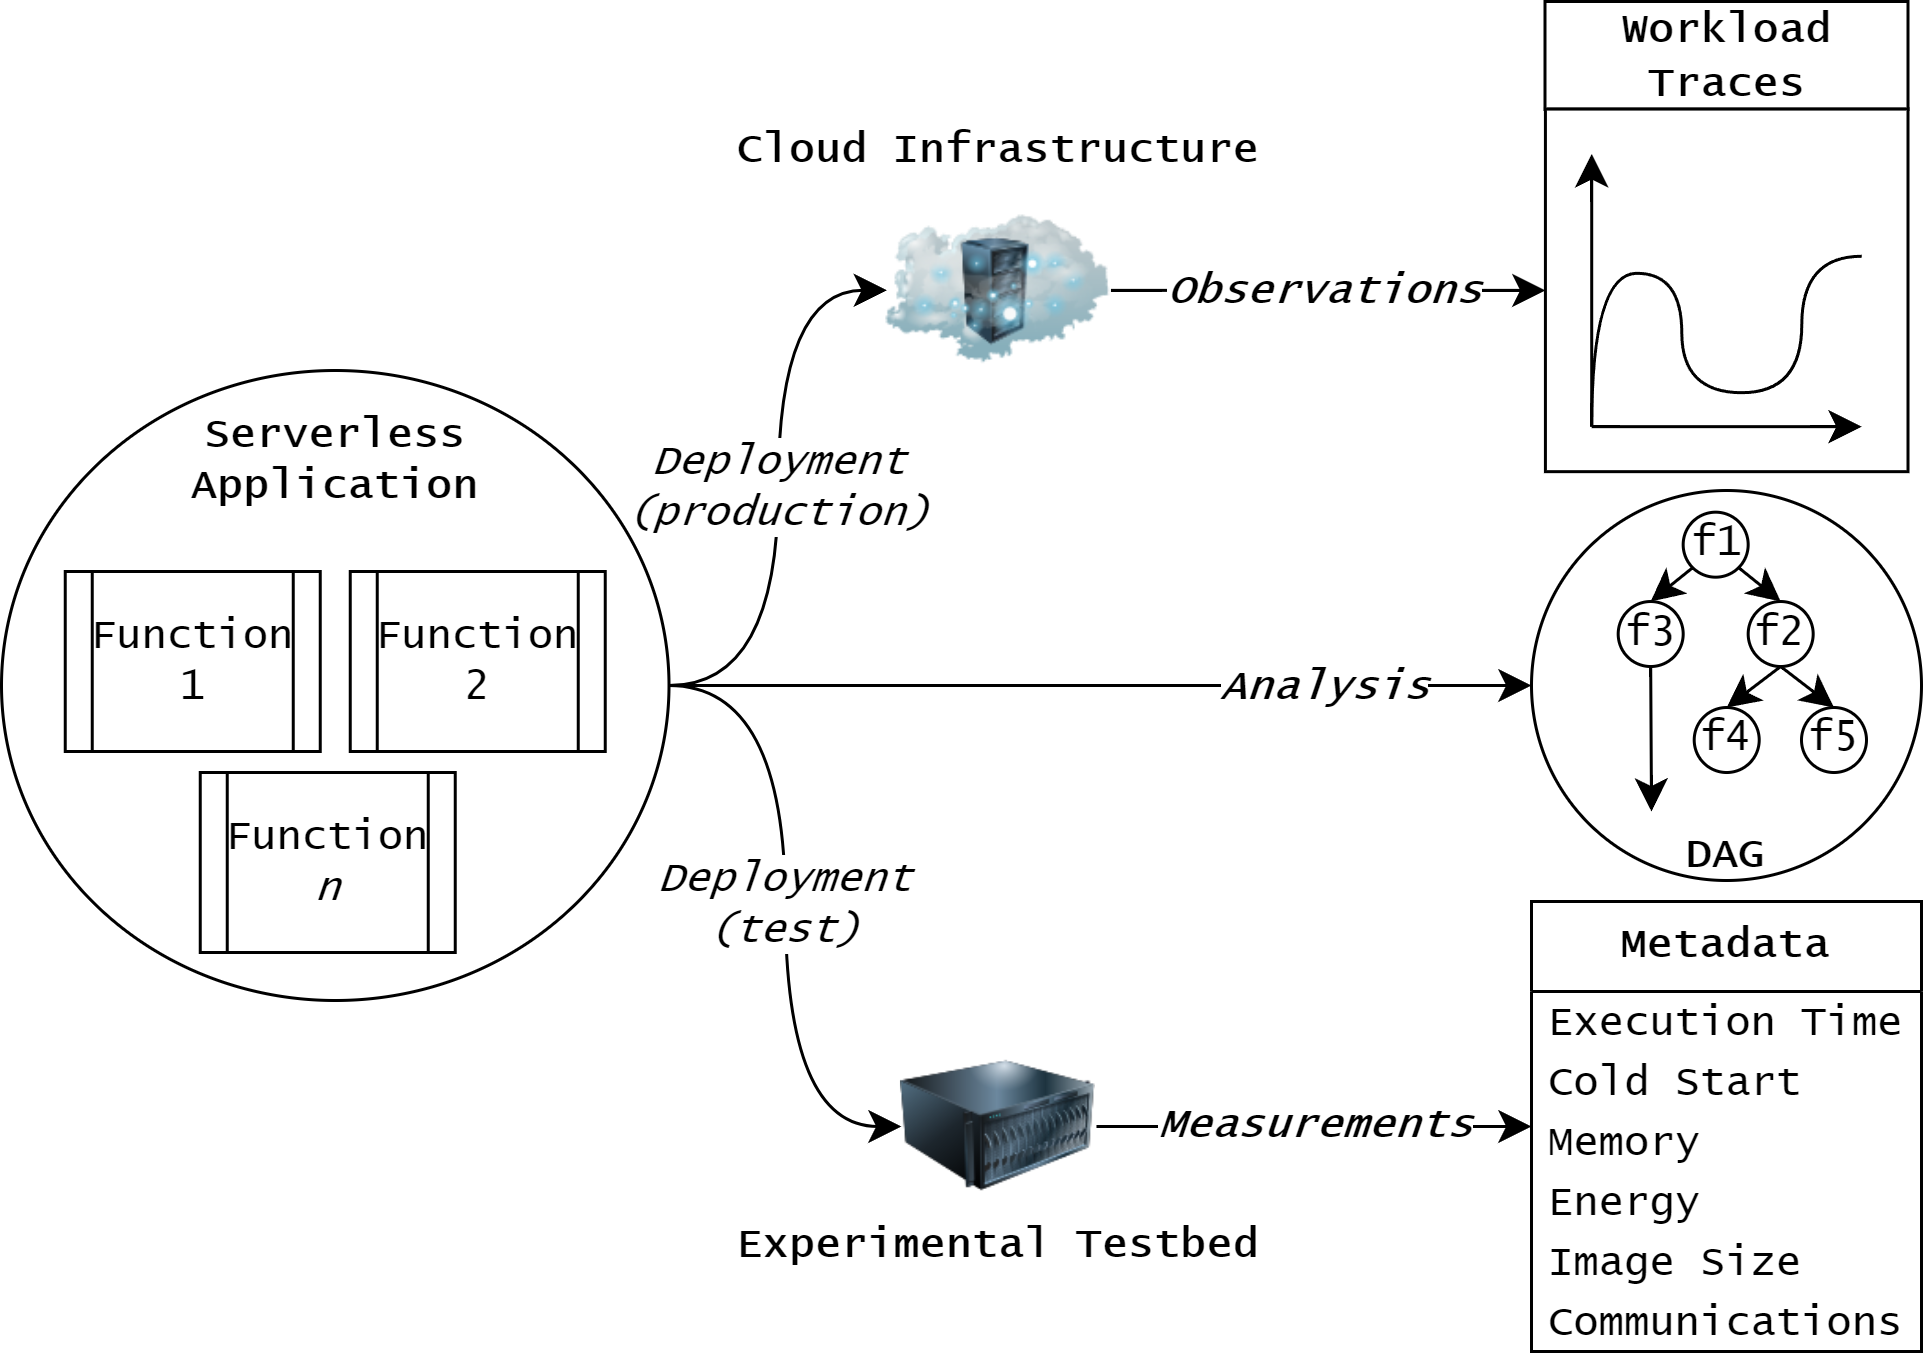
\includegraphics[width=\columnwidth]{7_Chapitre5/figures/characterization.png}
%     \caption{An overview of our characterization methodology.}
% \label{figure:herosim-characterization}
% \end{figure}

%During the simulation, logs are written to the disk. When all the user requests have been processed, the simulation stops and returns results and charts summarizing the simulation run. \vl{c'est expliqué dans User Interface, on peut le retirer ici} %, respectively in the \texttt{result} and \texttt{chart} directories.





%The simulator is single-threaded, meaning that each policy will be evaluated sequentially. However, multiple instances of HeROsim can be run in parallel with different configurations across multiple CPU cores, or distributed across multiple nodes. With every HeROsim instance running a different orchestration policy, and all instances using a common output directory, this can accelerate the total makespan of the simulation scenario when evaluating numerous orchestration policies. When all the simulator runs are finished, results can be consolidated in a single charts output. \jb{je pense que ce paragraphe peut sauter si manque de place, rien de très interessant}

\subsection{Orchestrateur}

The base \textbf{\texttt{Orchestrator}} class provides abstract initialization methods that are to be overridden to manage different structures of system state. For example, a Round Robin scheduler would need to know how many times each function replica has been selected for task placement, while a Least Connected scheduler will need to know the average concurrency in each replica to balance the load. This class is the entry point for users to define their own data structures that will best represent the system state to feed the \texttt{Autoscaler} and \texttt{Scheduler} to manage.

Users can implement the system state management process they need to support their orchestration policies. The base orchestrator is provided with a simple system that can serve as-is, or be extended. %as an example for more advanced techniques. 
In our implementation, a monitoring process is called periodically to keep track of the average concurrency in each function replica. This is useful for threshold-based policies.

The orchestrator entrypoint method is called each time a user request hits the platform. It takes the system state and the user request as input. It can be overridden in each orchestration policy implementation to enable fine-grained autoscaling and scheduling as needed.

Finally, this class is responsible for instantiating the selected implementations of \texttt{Autoscaler} and \texttt{Scheduler}. Any combination of these two modules can work together.

%\jb{pour chaque module plus bas, il manque une information claire indiquant quelles stratégies sont impléménentées par ce module. Peut être rajouter une phrase à la fin de chaque module pour dire voila les stratégies implémentées.}\vl{done}
\subsection{Allocateur}

The base \textbf{\texttt{Autoscaler}} class provides the common behavior of the autoscaling platform, including the creation and removal of function replicas. Several abstract methods have to be overridden to implement a new policy: resource selection for replica creation, replica initialization process, replica selection for removal, etc. These methods operate at the granularity of a single function, taking the system state and the list of available hardware resources as input. %Users are free to implement whichever algorithms they wish to evaluate for resource management.

HeROsim's autoscaler was primarily designed for horizontal scaling. Function replicas are created by allocating one execution platform and the required amount of peak memory on a node. An execution platform cannot host more than one function replica at a time. To accommodate higher load on an application without QoS degradation, new function replicas need to be allocated by the autoscaler, provided that enough hardware resources are available. Newly allocated replicas will go through an initialization phase during which function images have to be retrieved through the network. The autoscaler can manage an image cache in node memory and on node-local storage to accelerate cold starts.

Removing idle replicas is done on a best-effort basis: the autoscaler tries to remove replicas with empty task queues. By default, a replica with pending tasks cannot be removed.

The autoscaler keeps track of each allocation event to compute resource usage at the end of the simulation. HeROsim allows the user to know which nodes and execution platforms have been enrolled during the scenario, at which time and for which duration, and for which function deployment they were chosen. This also enables HeROsim to compute energy consumption at different granularities: static power needed by allocated hardware, and dynamic power used by applications during their execution.

HeROsim ships with the following concurrency threshold-based ready-to-use autoscaling policies:

\begin{itemize}
    \item Random -- Selects a random node and execution platform for new replicas.
    \item Knative -- Selects the least loaded node to allocate new replicas, \textit{i.e.} balances workloads across a large number of nodes.
    \item HeROfake -- Leverages hardware heterogeneity to minimize QoS penalties, energy consumption and Total Cost of Ownership. %More details are given in the "Case study" section.
    \item HeROcache -- Optimizes allocations for functions chains; maximizes consolidation functions of each application. %More details are given in the "Case study" section.
\end{itemize}

\subsection{Ordonnanceur}

The base \textbf{\texttt{Scheduler}} class implements task selection in the gateway queue. One abstract method has to be overridden to implement a new policy: the selection of replica among the pool to place each user request in queue. This method operates at the granularity of one user request and takes the system state and the list of available function replicas as input.

User requests arrive in a queue at the scheduler level. Users can implement their own priority policy for task selection, or choose a policy already available in the simulator, \textit{e.g.} FIFO or Earliest Deadline First~\cite{herofake}.

HeROsim's scheduler has been designed without task failure or migrations in mind: the default behavior considers tasks that always run to completion on their replica. However, tasks will be marked as "in penalty" if scheduling misses their deadline. Users can leverage this boolean value to evaluate the quality of their policies with regard to request latency: it indicates what proportion of requests are handled in a timely fashion. 

%If there is no replica available at the time of scheduling a user request, the scheduler will make a call to the autoscaler to force the creation of a first replica for the function. In the meantime, the request will be put back in queue and postponed. Postponed tasks are flagged as such, so that, for instance, they can have higher priority if the user wants to enforce such a policy~\cite{herocache}. \vl{paragraphe pas forcément indispensable ? c'est un "cas particulier" (scale from zero) de l'autoscaler}

HeROsim ships with the following scheduling policies implemented and ready to use:

\begin{itemize}
    \item Random -- Selects a random replica for task placement.
    \item Knative -- Selects the replica with the shortest in-flight request queue for task placement.
    \item BPFF -- Selects the replica with the longest in-flight request queue for task placement.
    \item HeROfake -- Selects the replica that minimizes a compound score according to the task's deadline, energy consumption of the function and scattering of tasks across nodes. %More details are given in the "Case study" section.
    \item HeROcache -- Selects the replica similar to HeROfake, but takes the storage and commuincation into account. %operations into account to compute the request's end-to-end latency, and takes the functions chains into account when scoring replicas with regards to tasks consolidation. %More details are given in the "Case study" section.
\end{itemize}


\subsection{Interface utilisateur}

%Interactions between the user and the simulator are limited. 
HeROsim relies on logging to provide insight as to how the simulation unwinds, helping the user debug their policies. When the simulation ends, result files are saved to disk. These files contain digest information on the results of the simulation, including the performance of the policy with regards to evaluation metrics. These results are plotted on various charts that can be used in further publications (see Figure~\ref{figure:herosim-evaluation}). HeROsim can also plot cold starts, cache hits and tail latency at the granularity of user requests. %\vl{viré le paragraphe dessous et résumé en 1 phrase}

% HeROsim can also generate additional charts that can be of use when debugging the behavior of an orchestration policy. Users can visualize the proportion of cold starts and cache hits across function invocations. HeROsim can plot tail latency for all user requests, helping the user rightsize their infrastructure. The execution trace generator will plot requests inter-arrival times on a chart to provide visual cues on the characteristics of the workload.

%There is ongoing work on extending HeROsim to propose a web interface to visualize the simulation state in real time. This interface might be shipped with a future version of the simulator.

\begin{figure}[t]
    \centering
    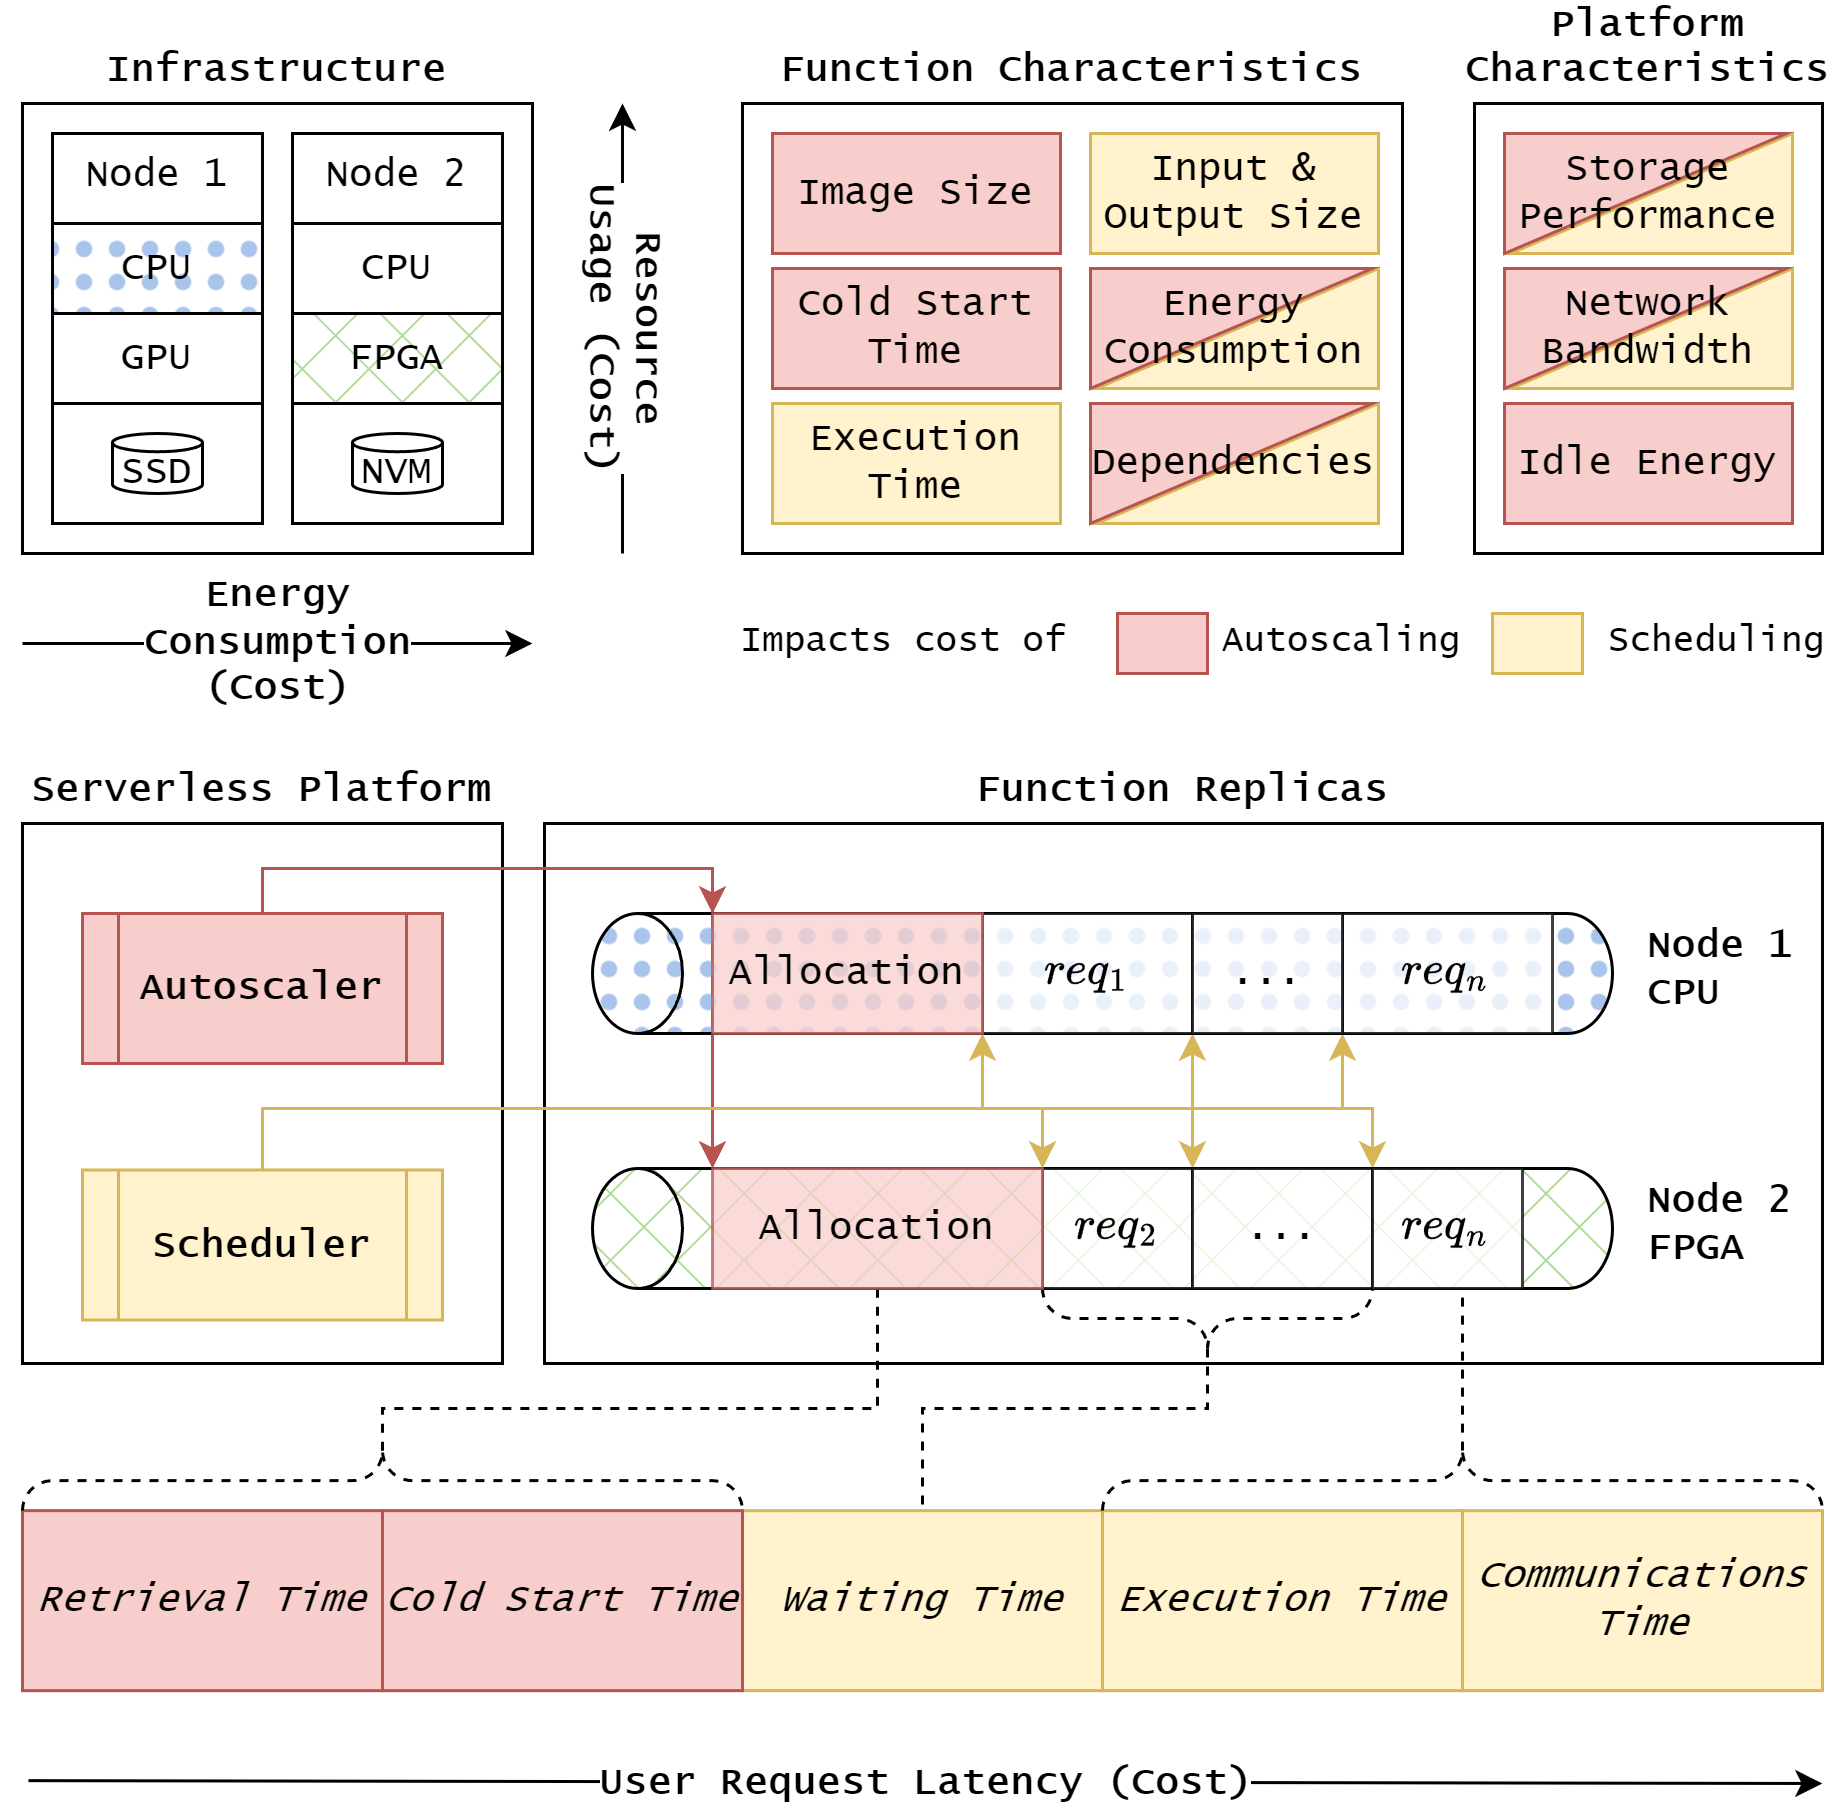
\includegraphics[width=\columnwidth]{7_Chapitre5/figures/serverless-cost.png}
    \caption{Breakdown of the end-to-end latency cost incurred by autoscaling and scheduling decisions.}
\label{figure:herosim-cost}
\end{figure}

\section{Étude de cas}
\label{section:herosim-case-study}

%\jb{je ne m'attendais pas à cela dans la section case study. Je m'attendais plutôt à une section plus conséquente ou l'on donne clairement comment passer du pb à la mise en oeuvre sur le simulateur avec un peu plus de détails techniques. la, ça fait un peu commercial, on donne juste les résultats}\vl{section complètement réécrite}

\begin{figure*}[t]
    \center
    \subfloat[Consolidation\label{figure:herosim-evaluation-full-unused-nodes}]{
        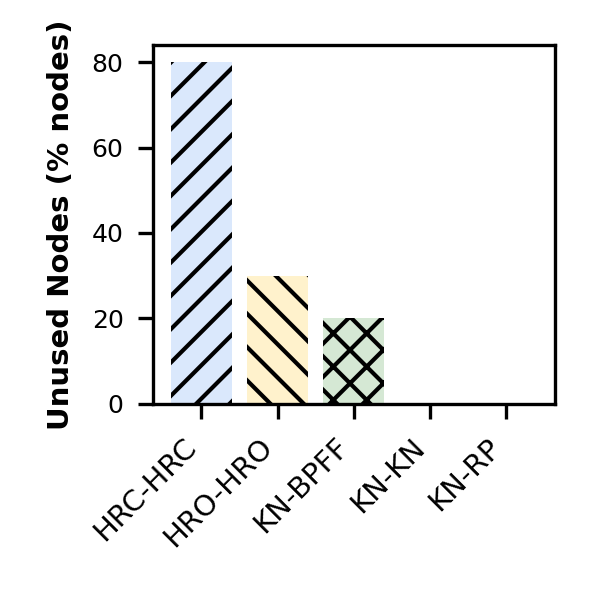
\includegraphics[width=0.155\linewidth]{7_Chapitre5/figures/eval/2-unused-nodes.png}
    }
    \subfloat[QoS\label{figure:herosim-evaluation-full-penalty}]{
        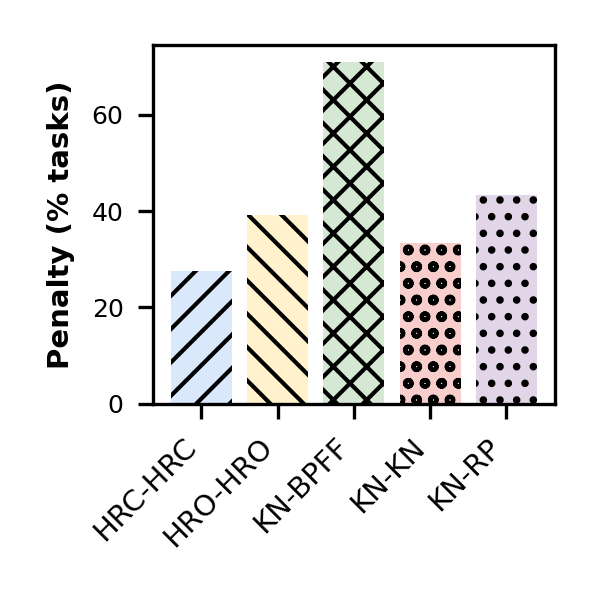
\includegraphics[width=0.155\linewidth]{7_Chapitre5/figures/eval/3-penalty-proportions.png}
    }
    \subfloat[Energy\label{figure:herosim-evaluation-full-energy-consumption}]{
        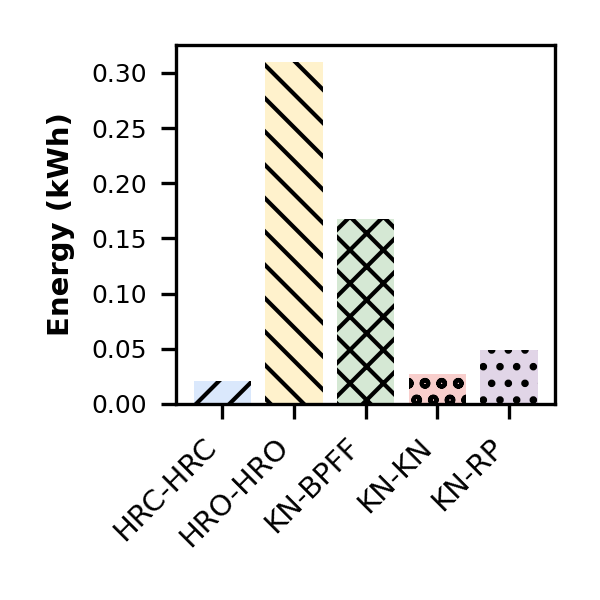
\includegraphics[width=0.155\linewidth]{7_Chapitre5/figures/eval/6-energy-consumption.png}
    }
    \subfloat[Consolidation\label{figure:herosim-evaluation-components-unused-nodes}]{
        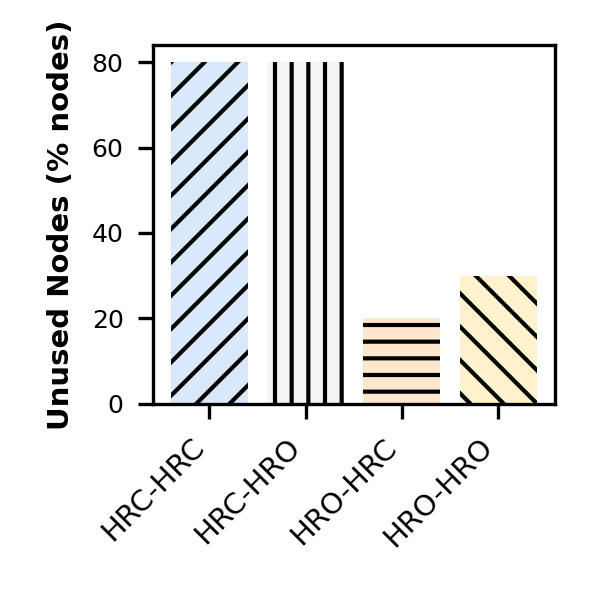
\includegraphics[width=0.155\linewidth]{7_Chapitre5/figures/eval-components/2-unused-nodes.png}
    }
    \subfloat[QoS\label{figure:herosim-evaluation-components-penalty}]{
        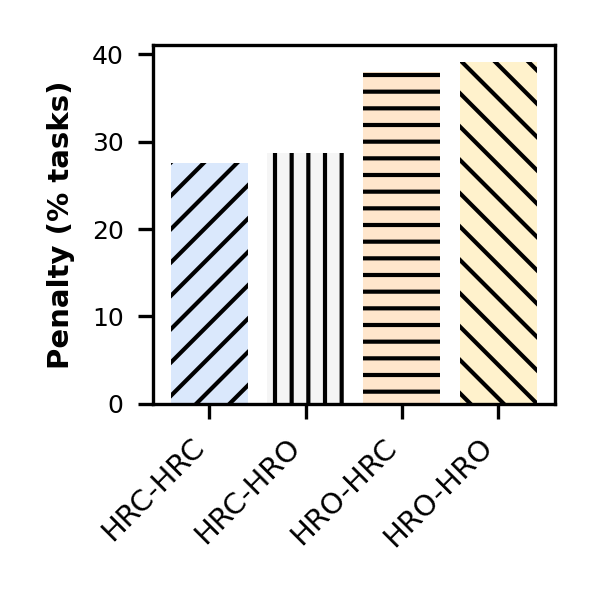
\includegraphics[width=0.155\linewidth]{7_Chapitre5/figures/eval-components/3-penalty-proportions.png}
    }
    \subfloat[Energy\label{figure:herosim-evaluation-components-energy-consumption}]{
        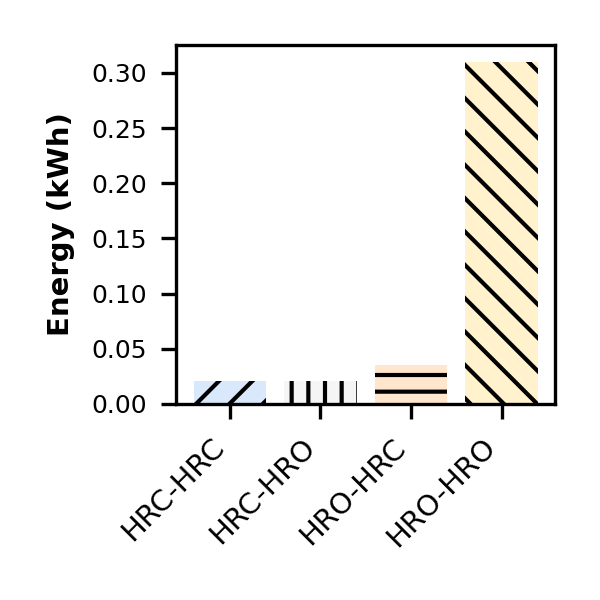
\includegraphics[width=0.155\linewidth]{7_Chapitre5/figures/eval-components/6-energy-consumption.png}
    }
    \caption{Charts generated by HeROsim for the evaluation of HeROcache -- Comparison against baselines (a-c) and impact of individual components (d-f). HRC-HRO means HeROcache autoscaler coupled with HeROfake scheduler.}
    \label{figure:herosim-evaluation}
\end{figure*}

%This simulation tool has been developed to support research work on orchestration policies in private serverless cloud. We argued that various challenges limit the relevance of serverless for users, and hinders the cost efficiency of the model for service providers:

% \begin{itemize}
%     \item The absence of QoS guarantees in serverless platforms prevents meeting the users' requirements in different use cases~\cite{Lannurien2023}.
%     \item Serverless platforms consider the underlying infrastructure as homogeneous and miss on the opportunity to further optimize task placements~\cite{herofake}.
%     \item Most orchestrators do not consider the costs linked with storage operations that can dominate functions' execution time~\cite{herocache}.
% \end{itemize}

%We investigated the design of a serverless platform that would tackle these challenges. Implementing the software necessary for our experiments would have been time-consuming, hence resorting to simulation was considered a more cost-efficient approach.

We present two case studies that made use of HeROsim to evaluate orchestration policies.
We devised strategies that rely on heterogeneous platform and workload characterization. % (see Figure~\ref{figure:herosim-characterization}).
%We measured several metrics related to our applications on various hardware platforms. 
We proposed a cost model that integrates these values to estimate the performance of autoscaling and scheduling under different policies, see Figure~\ref{figure:herosim-cost}.

% In both studies, we used HeROsim to evaluate our policies against various baselines, as well as to individually measure the impact of different autoscaler and scheduler configurations. Figure~\ref{figure:herosim-evaluation} shows the output charts that the simulator generated while evaluating HeROcache.



%\jb{dans ton intro, tu as indiqué des critères qu'un simulateur doit avoir. il faudrait dans la partie case study, dire dans des section séparaées comment chaque critère est pris en compte par case study. Je pense que ça serait interessant.}\vl{done}

\subsection{HeROfake}
% TODO: On-demand deepfake detection (inference tasks)
% TODO: Stateless tasks, no dependencies

In this first case study, \textbf{He}terogeneous \textbf{R}esources \textbf{O}rchestration for deep\textbf{fake} detection~\cite{herofake}, we investigated the deployment of a deepfake detection application on a serverless platform in a private cloud. %In particular, we were interested in leveraging heterogeneous resources for serverless orchestration when optimizing the platform for QoS and energy consumption.

The application runs inference tasks to detect deepfakes in potentially tampered-with images, submitted by users with various QoS level requirements. % Its objective is to detect potentially tampered-with images; pictures that might have been computer-manipulated to mislead viewers.
It consists of three independent and stateless neural network tasks that were implemented on heterogeneous hardware: CPU, GPU and FPGA. %These implementations were used for measurements.%, but it would have been challenging to actually run real-world scenarios on a serverless platform including these hardware architectures.

% TODO: Challenges: per-request QoS requirements, leverage heterogeneous hardware, scarcely available, actual executions impossible

%HeROfake did not consider applications (functions chains), hence user requests corresponded to single task executions. 
In HeROfake, each task execution has an associated cost measured in \textbf{latency}. Allocating new replicas on idle hardware resources introduces a \textbf{cold start delay}; handling user requests on different hardware has various \textbf{function execution time}. Latency for each user request is ultimately compared with the request's \textbf{QoS requirement}: if the request deadline was missed, the task is in \textbf{penalty}. These elements constitute the basis of our cost model, see Figure~\ref{figure:herosim-cost}.

% TODO: Strategy: cost minimization, heterogeneous threshold-based autoscaling, EDF scheduling

Different hardware architectures also have different monetary and energy costs that were factored in the cost model. We implemented an autoscaler and a scheduler policy that seek to estimate and minimize this composite cost at the granularity of each user request. The autoscaler seeks to allocate platforms that minimize the overall cost, including resource usage, energy consumption and Total Cost of Ownership. The scheduler seeks to select replicas that handle requests with least penalties and lowest energy consumption.

% TODO: Scenario

% TODO: HeROfake was evaluated using a synthetic scenario with uniform distribution of request inter-arrival times, function calls and QoS levels.

% TODO: Results

%HeROfake proved to perform well (in terms of QoS penalties, consolidation, and energy) against Knative (Google's serverless orchestrator) and Bin-Packing First Fit (Amazon's policy in Lambda)~\cite{herofake}. 

%Our main goal was to investigate the relevance of taking hardware heterogeneity into account when allocating resources and scheduling user requests with regards to various QoS metrics, \textit{i.e.} end-to-end latency and energy consumption.

%Experimental results showed that while total task execution time in HeROfake is similar to vanilla Knative, we achieve more than 60\% reduction in QoS penalties; tasks are consolidated on less than 40\% of the infrastructure's nodes, with 77\% execution platforms left unused; and dynamic energy consumption is reduced by 35\% as compared to Knative.

%HeROsim also allowed us to evaluate the impact of the individual components of our framework. Results showed that, even allocating CPUs only, scheduling inference tasks with our QoS-aware policy could keep SLA violations under 50\%. 


\subsection{HeROcache}

% TODO: Intermittent intrusion detection (pre-processing and inference tasks)

Here, a \textbf{He}terogeneous \textbf{R}esources \textbf{O}rchestration with a \textbf{cache} strategy for a storage-aware execution was deisgned. We explored the deployment of an Intrusion Detection System (IDS) on a serverless platform. In particular, we explored the benefits of data-aware orchestration when leveraging heterogeneous hardware to deploy time-sensitive applications on resources-constrained edge devices.%, from the perspective of the service provider.


%The goal of the application is to detect potentially malicious TCP traffic in user-submitted networking logs. As this IDS application is specifically targeted at drones missions, its access pattern is tightly related to seasonal patterns that make it a good fit for the serverless paradigm.

% TODO: Stateful application, temporal and data dependencies

The application consists of two layers: two preprocessing functions that operate on logs of network traffic, and four inference functions that detect patterns of malicious activity in the logs. These functions have been implemented on various edge hardware architectures (CPUs, FPGA, GPU). 

% TODO: Challenges: dependencies between functions, resources-constrained edge nodes, slow communications through remote storage, node-local storage contention (function cache vs intermediate data storage)
There are data dependencies between the two layers of the application. We modeled them as a Directed Acyclic Graphs (DAG) of function calls. % We used Python's \texttt{TopologicalSorter} from the \texttt{graphlib} module for JSON representation of the graphs and to traverse them during runtime.

%At the orchestrator level, we had to change the granularity of user requests: a user request concerns an application, which can be made up of one or more functions, called in the order defined by the application's DAG. Each function can take input data and produce output data. These data are defined by their size in bytes.

% TODO: Strategy: consolidation of applications' functions to minimize remote storage use, dependencies pre-fetching in cache for cold start acceleration

While HeROfake did not consider storage operations, HeROcache implements \textbf{function image retrieval}, \textbf{function image caching} and \textbf{inter-function communications} in the base orchestrator. These operations add up to user request latency by an amount of time computed on the basis of platform and function characterization, see Figure~\ref{figure:herosim-cost}. %: for example, HeROsim estimates function image retrieval time based on the network bandwidth specified by the user in the infrastructure description, the function image size specified by the workload type, and the node-local storage performance specified by the storage type.

%Introducing storage operations at individual node level allowed us to evaluate a function image prefetching strategy to accelerate cold starts in future invocations.

In HeROcache, the autoscaler seeks increased function consolidation across applications, reduced overall makespan, energy consumption and Total Cost of Ownership. The scheduler seeks to avoid missed request deadlines, use less power and enforce high resource usage.

% TODO: Workload characterization, synthetic workload trace based on a Poisson process, 4G LTE request rate

% We used the execution trace generator included in HeROsim to generate a 30-minute scenario of user requests following a Poisson process at an average rate of 83 Requests per Second. This corresponds to the rate of communications that 4G LTE connectivity would allow in our edge setting, given the size of the application input and output data. 

% TODO: Results

Evaluation against HeROfake highlighted the relevance of taking into account storage operations, see Figure~\ref{figure:herosim-evaluation}.

% We evaluated HeROcache against various baselines (Knative, BPFF, RP) and also against HeROfake, see Figure~\ref{figure:herosim-evaluation}.

%As HeROfake already leveraged hardware heterogeneity but was designed as a storage-oblivious policy, it made for a comparable solution. 
%This comparison allowed us to show the relevance of storage costs in QoS compliance  %showed that, with a data-aware orchestration policy, HeROcache enforces applications consolidation and manages to reduce average initialization delays by 17.6\% and communication delays by 88.4\%. This results in reducing the static energy consumption of the platform by 80\% while maintaining under 28\% of QoS violations.\jb{on peut raccourcir je pense}

%HeROcache (implemented on top of HeROsim) has been submitted for artifacts evaluation and received the three IEEE reproducibility badges~\footnote{\href{https://www.niso.org/standards-committees/reproducibility-badging}{https://www.niso.org/standards-committees/reproducibility-badging}}: Open Research Objects (ORO), Reusable/Research Objects Reviewed (ROR), and Results Reproduced (ROR-R).


% To address these issues, we proposed:
% \begin{itemize}
%     \item HeROfake~\cite{herofake}, a framework for the deployment of short-lived, interactive deepfake detection tasks on a private, heterogeneous serverless cloud. Experimental results showed that while total task execution time in HeROfake is similar to vanilla Knative, we achieve more than 60\% reduction in QoS penalties; tasks are consolidated on less than 40\% of the infrastructure's nodes, with 77\% execution platforms left unused; and dynamic energy consumption is reduced by 35\% as compared to Knative.
%     \item HeROcache~\cite{herocache}, an allocation and scheduling policy for serverless edge computing that seeks to optimize time-sensitive applications deployment for QoS on energy-constrained devices. HeROcache enforces applications consolidation and manages to reduce average initialization delays by 17.6\% and communication delays by 88.4\%. This results in reducing the static energy consumption of the platform by 80\% while maintaining under 28\% of QoS violations.
% \end{itemize}

\section{Travaux connexes}
\label{section:herosim-sota}
%\jb{c'est TROOOP long !!!, ce n'est pas les related work qui feront que le papier sera accepté, une colonne c'set amplement suffisant. Il faut renforcer la contrib et le case study absolument !!} \vl{ok, on raccourcira à la fin, ce sera facile. j'ai détaillé chaque contrib et je les ai aussi regroupées par caractéristique. On peut garder uniquement les regroupements et virer les détails individuels.}\jb{ok} \vl{done, j'ai gardé les grandes familles (CloudSim, GridSim), j'ai fait les regroupements qui me semblaient pertinents et j'ai raccourci la section à environ une colonne}

\begin{table*}[t]
    \centering
    \caption{Overview of simulation tools for cloud computing}
    \resizebox{\linewidth}{!}{
        \begin{tabular}{lSSSSSSSSS}
        \toprule
        & Serverless & Deployment models & Functions chains & Hardware heterogeneity & Per-request QoS & Resource usage & Energy consumption & Visualization \\
        \cmidrule(lr){2-2}\cmidrule(lr){3-3}\cmidrule(lr){4-4}\cmidrule(lr){5-5}\cmidrule(lr){6-6}\cmidrule(lr){7-7}\cmidrule(lr){8-8}\cmidrule(lr){9-9}
        CloudSim~\cite{calheiros_cloudsim_2011} & \xmark & Public, private, hybrid & \xmark & \cmark & \xmark & \cmark & \cmark & \xmark \\
        CloudSimSC~\cite{mampage_cloudsimsc_2023} & \cmark & Public, private, hybrid & \xmark & \cmark & \xmark & \cmark & \cmark & \xmark \\
        CloudAnalyst~\cite{wickremasinghe_cloudanalyst_2010} & \xmark & Public, private, hybrid & \xmark & \cmark & \xmark & \cmark & \cmark & \cmark \\        DFaaSCloud~\cite{jeonCloudSimExtensionSimulatingDistributed2019} & \cmark & Multi-tier hybrid cloud & \xmark & \xmark & \cmark & \cmark & \xmark & \cmark \\
        ElasticSim~\cite{cai_elasticsim_2017} & \xmark & Public & \cmark & \xmark & \xmark & \cmark & \xmark & \cmark \\
        GridSim~\cite{buyyaGridSimToolkitModeling2002} & \xmark & Grid & \xmark & \cmark & \cmark & \cmark & \xmark & \cmark \\
        iCanCloud~\cite{nunez_icancloud_2012} & \xmark & Public & \xmark & \xmark & \xmark & \cmark & \xmark & \cmark \\
        iFogSim2~\cite{mahmudIFogSim2ExtendedIFogSim2021} & \xmark & Edge, Fog & \xmark & \cmark & \xmark & \cmark & \cmark & \xmark \\
        OpenDC 2.0~\cite{mastenbroekOpenDCConvenientModeling2021} & \cmark & Public, private, hybrid & \cmark & \cmark & \xmark & \cmark & \cmark & \cmark \\
        SimFaaS~\cite{mahmoudiSimFaaSPerformanceSimulator2021} & \cmark & Public & \xmark & \xmark & \xmark & \cmark & \cmark & \cmark \\
        \textbf{HeROsim} & \cmark & Private & \cmark & \cmark & \cmark & \cmark & \cmark & \cmark \\
        \bottomrule
        \end{tabular}
    }
    \label{table:herosim-sota}
\end{table*}

We present an overview of state-of-the-art work and their characteristics in Table~\ref{table:herosim-sota}.

CloudSim~\cite{calheiros_cloudsim_2011} is the ubiquitous tool for large-scale cloud deployment experiments. It targets the different service models in traditional cloud computing. 
CloudSim, and its extensions~\cite{calheiros_cloudsim_2011, mampage_cloudsimsc_2023, wickremasinghe_cloudanalyst_2010, jeonCloudSimExtensionSimulatingDistributed2019} do not consider serverless applications, \textit{i.e.} the composition of functions to achieve complex behavior which introduces specific challenges.% (cold start delays, overhead from inter-function communications, etc.~\cite{wawrzoniakBoxerDataAnalytics2021a}). 
To address these particular problems, it is necessary to introduce storage management, as well as the handling of function chains as HeROsim does. % allows users to model such applications, and devise orchestration policies that are application-aware and can provide QoS benefits.

% DFaaSCloud~\cite{jeonCloudSimExtensionSimulatingDistributed2019} is another CloudSim-based simulator for distributed serverless computing. This work focuses on the geographical distribution of function instances across a cloud, edge and fog infrastructure. It helps estimating delays induced by function locality. Users define their functions in terms of latency constraints and DFaaSCloud provides a placement policy that minimizes violations and cost. As such, the premise of DFaaSCloud is specific to addressing the problem of geographical placement of tasks in a multi-tier Function as a Service environment, and does not pertain to the general challenges in serverless computing.

% ElasticSim~\cite{cai_elasticsim_2017} also extends CloudSim to provide dynamic resources allocation for cloud workflows, \textit{i.e.} chains of connected tasks not dissimilar to serverless applications. However, it does not consider the underlying heterogeneity in hardware resources, nor does it allow to enforce per-request QoS objectives. OpenDC 2.0~\cite{mastenbroekOpenDCConvenientModeling2021} also allows the user to model such function chains, and while this tool does allow modeling a heterogeneous datacenter and estimate its energy consumption, it also does not consider the variety of user requirements in terms of latency.

GridSim~\cite{buyyaGridSimToolkitModeling2002} has interesting characteristics, from modeling highly heterogeneous infrastructures to enforcing per-request QoS constraints. However, its focus on grid computing makes it unsuitable to explore dynamic resource allocation problems. iFogSim2~\cite{mahmudIFogSim2ExtendedIFogSim2021} also considers static allocations that cannot faithfully characterize the serverless problem space. HeROsim has been designed for the serverless problem space and allows users to trace dynamic allocation and scheduling events at a user request granularity.

Multiple contributions~\cite{jeonCloudSimExtensionSimulatingDistributed2019, cai_elasticsim_2017, buyyaGridSimToolkitModeling2002, nunez_icancloud_2012} do not allow one to estimate the energy consumption of the platform. 
%Energy consumption is a crucial metric when addressing the challenge of scheduling power-hungry computations such as Machine Learning (ML) training, which hold a growing proportion of deployed cloud workloads~\cite{masanet2020recalibrating}. 
HeROsim estimates both static energy consumption and dynamic energy consumption.

Furthermore, hardware heterogeneity is a defining characteristic in cloud computing. % Accelerators such as GPUs or TPUs are used by service providers to provide better performance.
% We argued that such hardware could allow service providers to enforce QoS constraints while reducing energy consumption of a serverless platform~\cite{herofake}.
Among the cloud simulation tools available, several contributions~\cite{jeonCloudSimExtensionSimulatingDistributed2019, cai_elasticsim_2017, nunez_icancloud_2012, mahmoudiSimFaaSPerformanceSimulator2021} do not take heterogeneity into account at a fine granularity. HeROsim lets users define highly heterogeneous infrastructures for both compute and storage.

Finally, some contributions~\cite{nunez_icancloud_2012, mahmoudiSimFaaSPerformanceSimulator2021} aim at simulating public cloud infrastructures that focus on the brokerage of virtualized resources that are considered unlimited. Our work~\cite{herofake, herocache} focused on the perspective of service providers optimizing serverless platforms for QoS, hence the private cloud orientation of HeROsim.


\section{Conclusion et perspectives}
\label{section:herosim-conclusion}

In this paper, we presented HeROsim, a simulation tool that aims at allowing researchers to model heterogeneous cloud infrastructures, describe workloads at a fine granularity, implement diverse resource management and task scheduling policies, and evaluate their efficiency with regard to metrics such as resource usage, energy consumption, per-request QoS violations, or tail latency. % HeROsim can generate charts that help visualizing these results during the implementation phase, and can be used in publications.

%There is ongoing work on extending HeROsim to propose a web interface to visualize the simulation state in real time. We are also working on a reinforcement learning agent that could be included in a future release.
% Also, we are working on the ability to run parallel simulations to reduce the simulation time.

%Our next contribution will leverage Q-Learning to explore the design of an autonomous agent which efficiently rightsizes resources allocations on the serverless platform. It will make use of time series prediction to allow timely, proactive autoscaling. This agent will be evaluated in the simulator, showcasing the variety of policies that can be implemented with our tool.
